\documentclass{beamer}
\usepackage{beamerthemeshadow}
\usepackage{xmpmulti}
\usefonttheme[onlymath]{serif}




\usecolortheme{rose}
\usetheme{Warsaw}


\title{Petaluma High School}
\author{Mr. Kelley}
\institute{Petaluma High School}
\date{Fall 2012}


\newcommand{\m}{\mbox{ m }}

\newcommand{ \bigLPic}[2]{
       \includegraphics[scale = .34]<#1>{#2}}

\newcommand{ \bigPPic}[2]{
       \includegraphics[angle = -90, scale = .20]<#1>{#2}}

\newcommand{ \halfnhalfLR}[2]{
       \begin{columns}
       \column{.5\textwidth}
       #1
       \column{.5\textwidth}
       #2
       \end{columns}
}
\newcommand{ \halfnhalfBR}[2]{
       \begin{columns}
       \column{.3\textwidth}
       #1
       \column{.7\textwidth}
       #2
       \end{columns}
}

\newcommand{ \halfnhalfBL}[2]{
       \begin{columns}
       \column{.7\textwidth}
       #1
       \column{.3\textwidth}
       #2
       \end{columns}
}

\newcommand{ \halfnhalfRL}[2]{
       \begin{columns}
       \column{.5\textwidth}
       #2
       \column{.5\textwidth}
       #1
       \end{columns}
}


\begin{document}

\section{Force}

\frame{
       \frametitle{Newton's Laws}
       \begin{center}
	These are principles by which we understand forces and motion. \pause \\ \emph{Everything can be related back to them.}
	\end{center}
}

\frame{
       \frametitle{First Law}
       
	An object will maintain constant velocity unless acted upon by an unbalanced force. \pause \\ What constitutes a change in velocity? \pause \\ What is an unbalanced force? \pause \\
	\begin{center}
	Mathematical Statement of the First Law:
	\end{center}
	$$\sum\limits_i \vec{F}_i = 0 \hspace{1cm} \Longrightarrow \hspace{1cm} \frac{\Delta \vec{v}}{\Delta t} = 0$$
}

\frame{
       	\frametitle{Second Law}
       	\pause
	The net force on an object is equal to the rate of change of its momentum. \\ \pause
	
	$$\sum\limits_i \vec{F}_i = \frac{\Delta \vec{\rho}}{\Delta t} \pause = \frac{d}{d t} (\vec{\rho})$$ \pause \vspace{1cm}
	$$\frac{\Delta \rho}{\Delta t} = \pause \frac{\Delta (mv)}{\Delta t} = \pause \frac{(m \Delta v)}{\Delta t} =\pause m \frac{\Delta v}{\Delta t} = \pause ma$$
	
	}
	
\frame{
       	\frametitle{Second Law}

	The net force on an object is equal to the product of the mass and acceleration of the object. \\ \pause
	
	$$\sum\limits_i F_i = ma$$ \pause \vspace{1cm}
	$$F = ma$$ \pause
	Know it\pause , use it\pause , love it.	
}

\frame{
       	\frametitle{Second Law}

	The net force on an object is equal to the product of the mass and acceleration of the object. \\ \pause
	
	$$\sum\limits_i F_i = ma$$ \pause \vspace{1cm}
	$$F = ma$$ \pause
	Know it\pause , use it\pause , love it.	
}

\frame{
       	\frametitle{Third Law}

	\begin{center}
	If object$_1$ acts on object$_2$ with a force $F$, then object$_2$ acts on object$_1$ with a force of $-F$. \\ \pause
	\vspace{1cm}
	``For every action there is an equal and opposite reaction."
	\end{center}
}

\frame{
	\frametitle{Applications}
       
	A 5 kg mass is at rest on a table.  What is the sum of the forces acting on it?  Draw a free-body diagram.
}

\frame{
	\frametitle{Applications}
       
	A 10 kg mass is hanging on a string.  What is the sum of the forces acting on it?  Draw a free-body diagram.
}


\frame{
       	\frametitle{Applications}
	Inertial Reference Frame
       	\begin{center}
	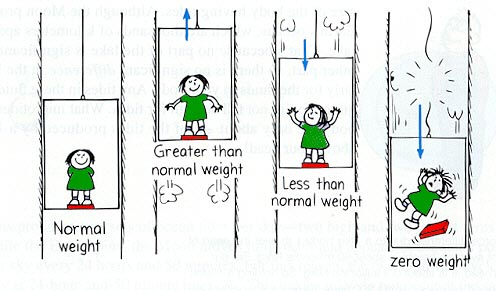
\includegraphics{elevator}
	\end{center}
}

\frame{
	\frametitle{Applications}
       
	A 10 kg mass is hanging on 2 strings.  What is the tension in each string?  Draw a free-body diagram.
}


\frame{
	\frametitle{Applications}
       
	A 10 kg mass is hanging on a clothesline.  If the clothesline makes an angle of 15$^\circ$ with the horizontal, what is the tension in the clothesline?
}

\frame{
	\frametitle{Applications}
       
	A 10 kg mass is being acted upon by two forces.  $\vec{F_1} = 12 N, 25^{\circ}$ and $\vec{F_2} = 20 N, 120^{\circ}$.  Draw a free-body diagram and find the direction and magnitude of the acceleration.
}

              
\end{document}